% STATUS: ACTIVE -- 2026-09-24 report. Title, model, figure; nothing else.
% Compile: xelatex 0924_report.tex   (from reference/eq17_analysis/derivation/)
% Figures: figures/fig_noap_ladder_lf1_only.png     plot_5state_noap_ladder({'ramp16'}, 5, {'_Td5_lf1'}, ...)
%          figures/fig_noap_vs_aprime_lf1_Td2.png   plot_5state_noap_vs_aprime_lf1
% Runs:    test_results/temp_5state_noap/ladder_ramp16_Td5_lf1_o{1,2}.mat, ladder_ramp16_Td2_lf1_o2.mat
%          test_results/temp_plaw_walls/f1p2_plane_PI_sig010_ramp2.mat
% Sections 3-5 (slope law a'(h; c, p)):
%          figures/obs_fixed_V_f1.png       probe_obs_fixed_height([], {'f1'})          cache test_results/temp_plaw_walls/obs_fixed_height_f1.mat
%          figures/obs_ramp_f1_V_Td2.png    probe_obs_ramp_f1(2, [], 'f1')              cache test_results/temp_plaw_walls/obs_ramp_f1_Td2.mat
%          figures/f1_walls_PI_ramp2.png    run_plaw_walls(law 'f1', traj 'ramp', Td 2) -> plot_plaw_walls('PI','_ramp2',{'plane','cell'},'f1')
%          runs: test_results/temp_plaw_walls/f1_{plane,cell}_PI_ramp2.mat (seeds 1:10)
% Sections 6-7 (slope law a'(h, c), p = 2, one constant):
%          figures/obs_ramp_f1p2_V_Td2.png           probe_obs_ramp_f1(2, [], 'f1p2')            cache test_results/temp_plaw_walls/obs_ramp_f1p2_Td2.mat
%          figures/f1p2_walls_PI_sig010_ramp2.png   run_plaw_walls(law 'f1p2', traj 'ramp', Td 2, sig 0.10, tag '_sig010') -> plot_plaw_walls('PI','_sig010_ramp2',{'plane','cell'},'f1p2')
%          runs: test_results/temp_plaw_walls/f1p2_{plane,cell}_PI_sig010_ramp2.mat (seeds 1:10)
% Section 9 (c-only slope law, cell wall, three forgetting factors on c):
%          figures/f1p2_cell_lf_compare.png          plot_f1p2_cell_lf_compare
%          runs: test_results/temp_plaw_walls/f1p2_cell_PI_sig010{_ib3,_lf999,}_ramp2.mat (run_lf_battery: lambda_f_b_info 3 / floor 0.99; lambda_f_b 0.999; lambda = 1)
\documentclass[11pt,a4paper]{ctexart}
\usepackage[fleqn]{amsmath}
\usepackage{amssymb,bm}
\setlength{\mathindent}{0pt}
\usepackage{geometry}
\geometry{margin=2.0cm}
\usepackage{graphicx}
\graphicspath{{figures/}}
\setlength{\parindent}{0pt}
\setlength{\parskip}{0.4em}
\pagestyle{plain}

\begin{document}

\begin{center}\textbf{\large 2026-09-24 report}\end{center}

Trajectory: hold 0.5 s, constant-velocity descent $22.2 \to 1.10\,R$ over $T_d$, hold 0.5 s. Plane. $\lambda_f = 1$. 5 seeds.

\section{First-order vs second-order gain model, $T_d = 5$ s}

\begin{align*}
\text{first order:}\quad  & a[k+1] = a[k] \\
\text{second order:}\quad & a[k+1] = a[k] + \delta a[k], & \delta a[k+1] &= \delta a[k]
\end{align*}

\begin{center}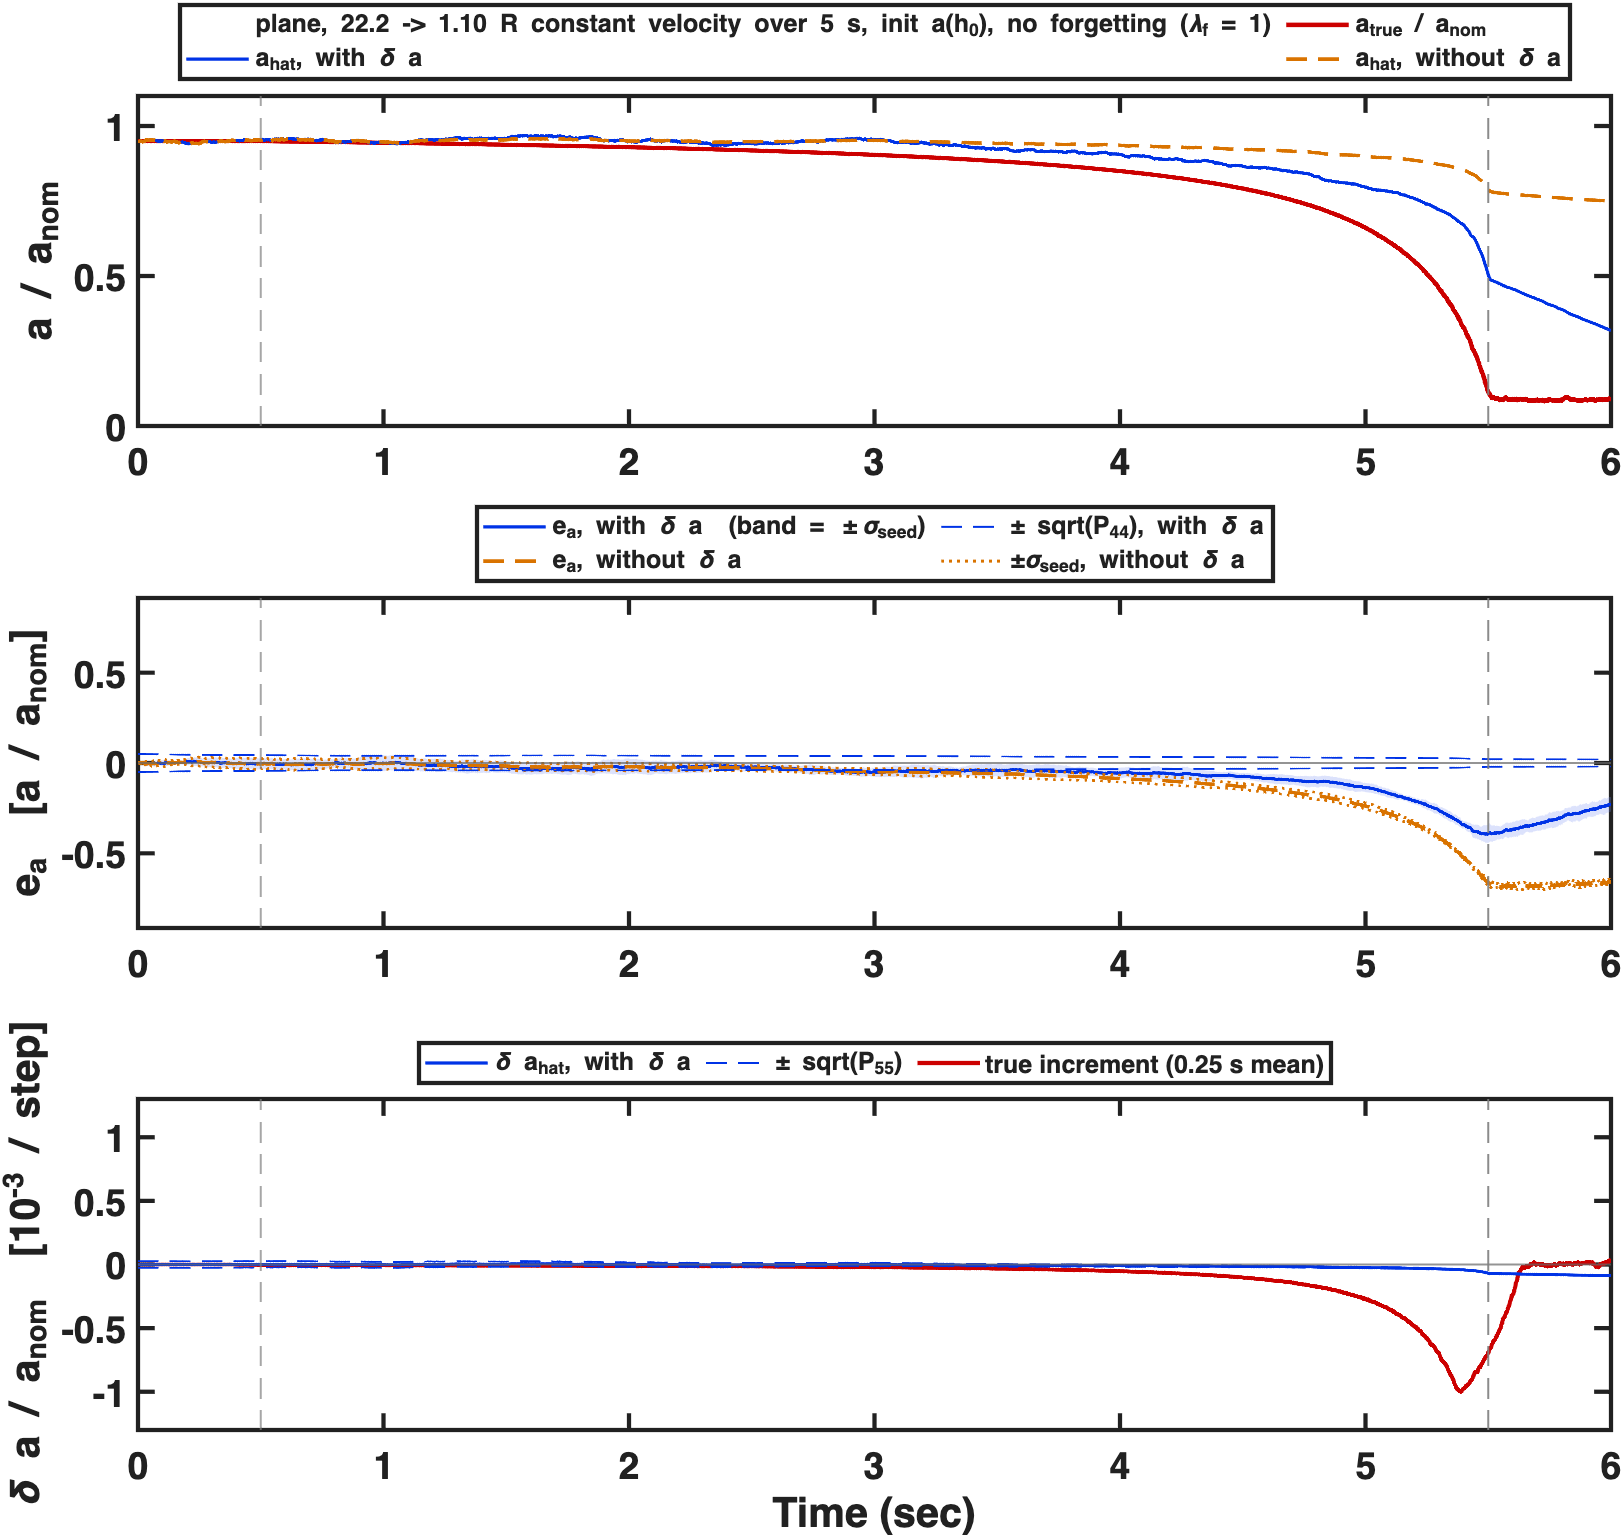
\includegraphics[width=0.9\textwidth]{fig_noap_ladder_lf1_only.png}\end{center}

\clearpage
\section{Second-order gain model vs slope law $a'(h, c)$, $T_d = 2$ s}

\begin{align*}
\text{second order:}\quad & a[k+1] = a[k] + \delta a[k], & \delta a[k+1] &= \delta a[k] \\
\text{slope law:}\quad    & a[k+1] = a[k] + a'(h_d[k], c)\,\Delta h_d[k], \quad a' = \frac{1-c}{h^2}, & c[k+1] &= c[k]
\end{align*}

\begin{center}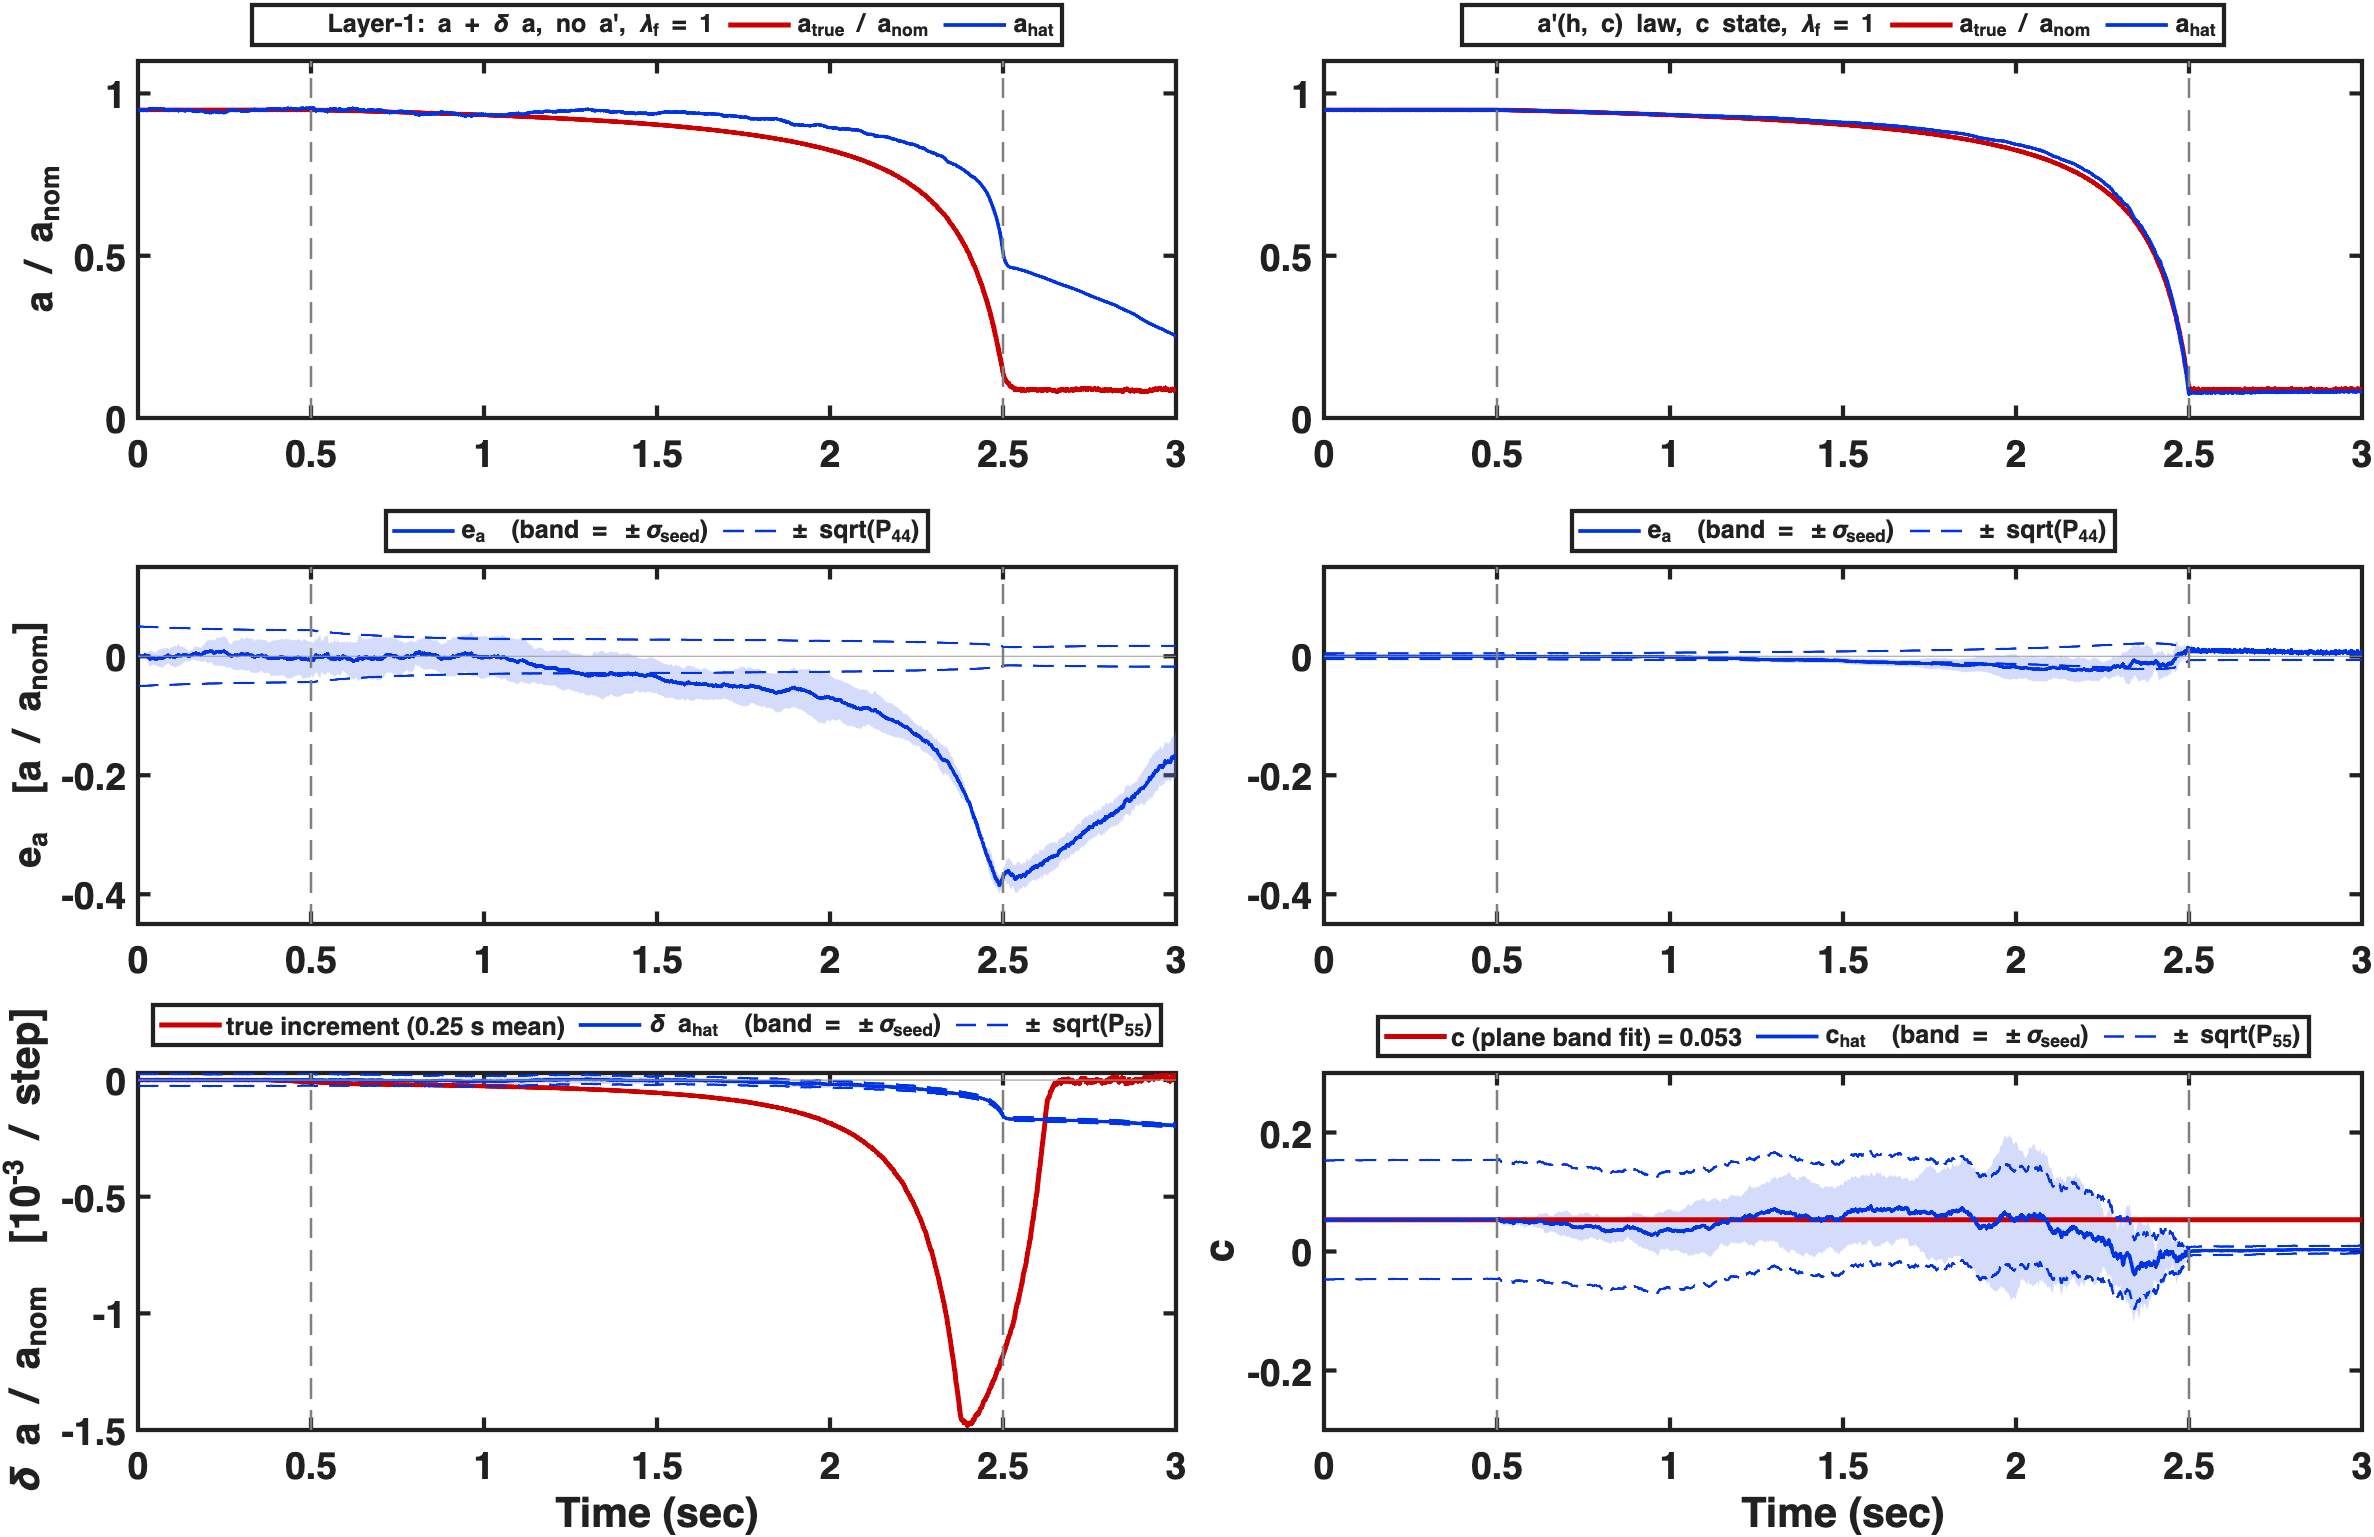
\includegraphics[width=\textwidth]{fig_noap_vs_aprime_lf1_Td2.png}\end{center}

\clearpage
\section{Slope law $a'(h;\,c,p)$, both constants estimated: fixed heights $22.2\,R$ and $1.10\,R$}

Plane and cell wall, plane init, held 3 s, one seed. $\sigma_i$, $v_i$: singular values and directions of the observability matrix over the run.
\begin{align*}
a[k+1] &= a[k] + a'(h_d[k];\,c,p)\,\Delta h_d[k], \qquad a' = \frac{1-c}{h^p} \\
c[k+1] &= c[k] \\
p[k+1] &= p[k]
\end{align*}

\begin{center}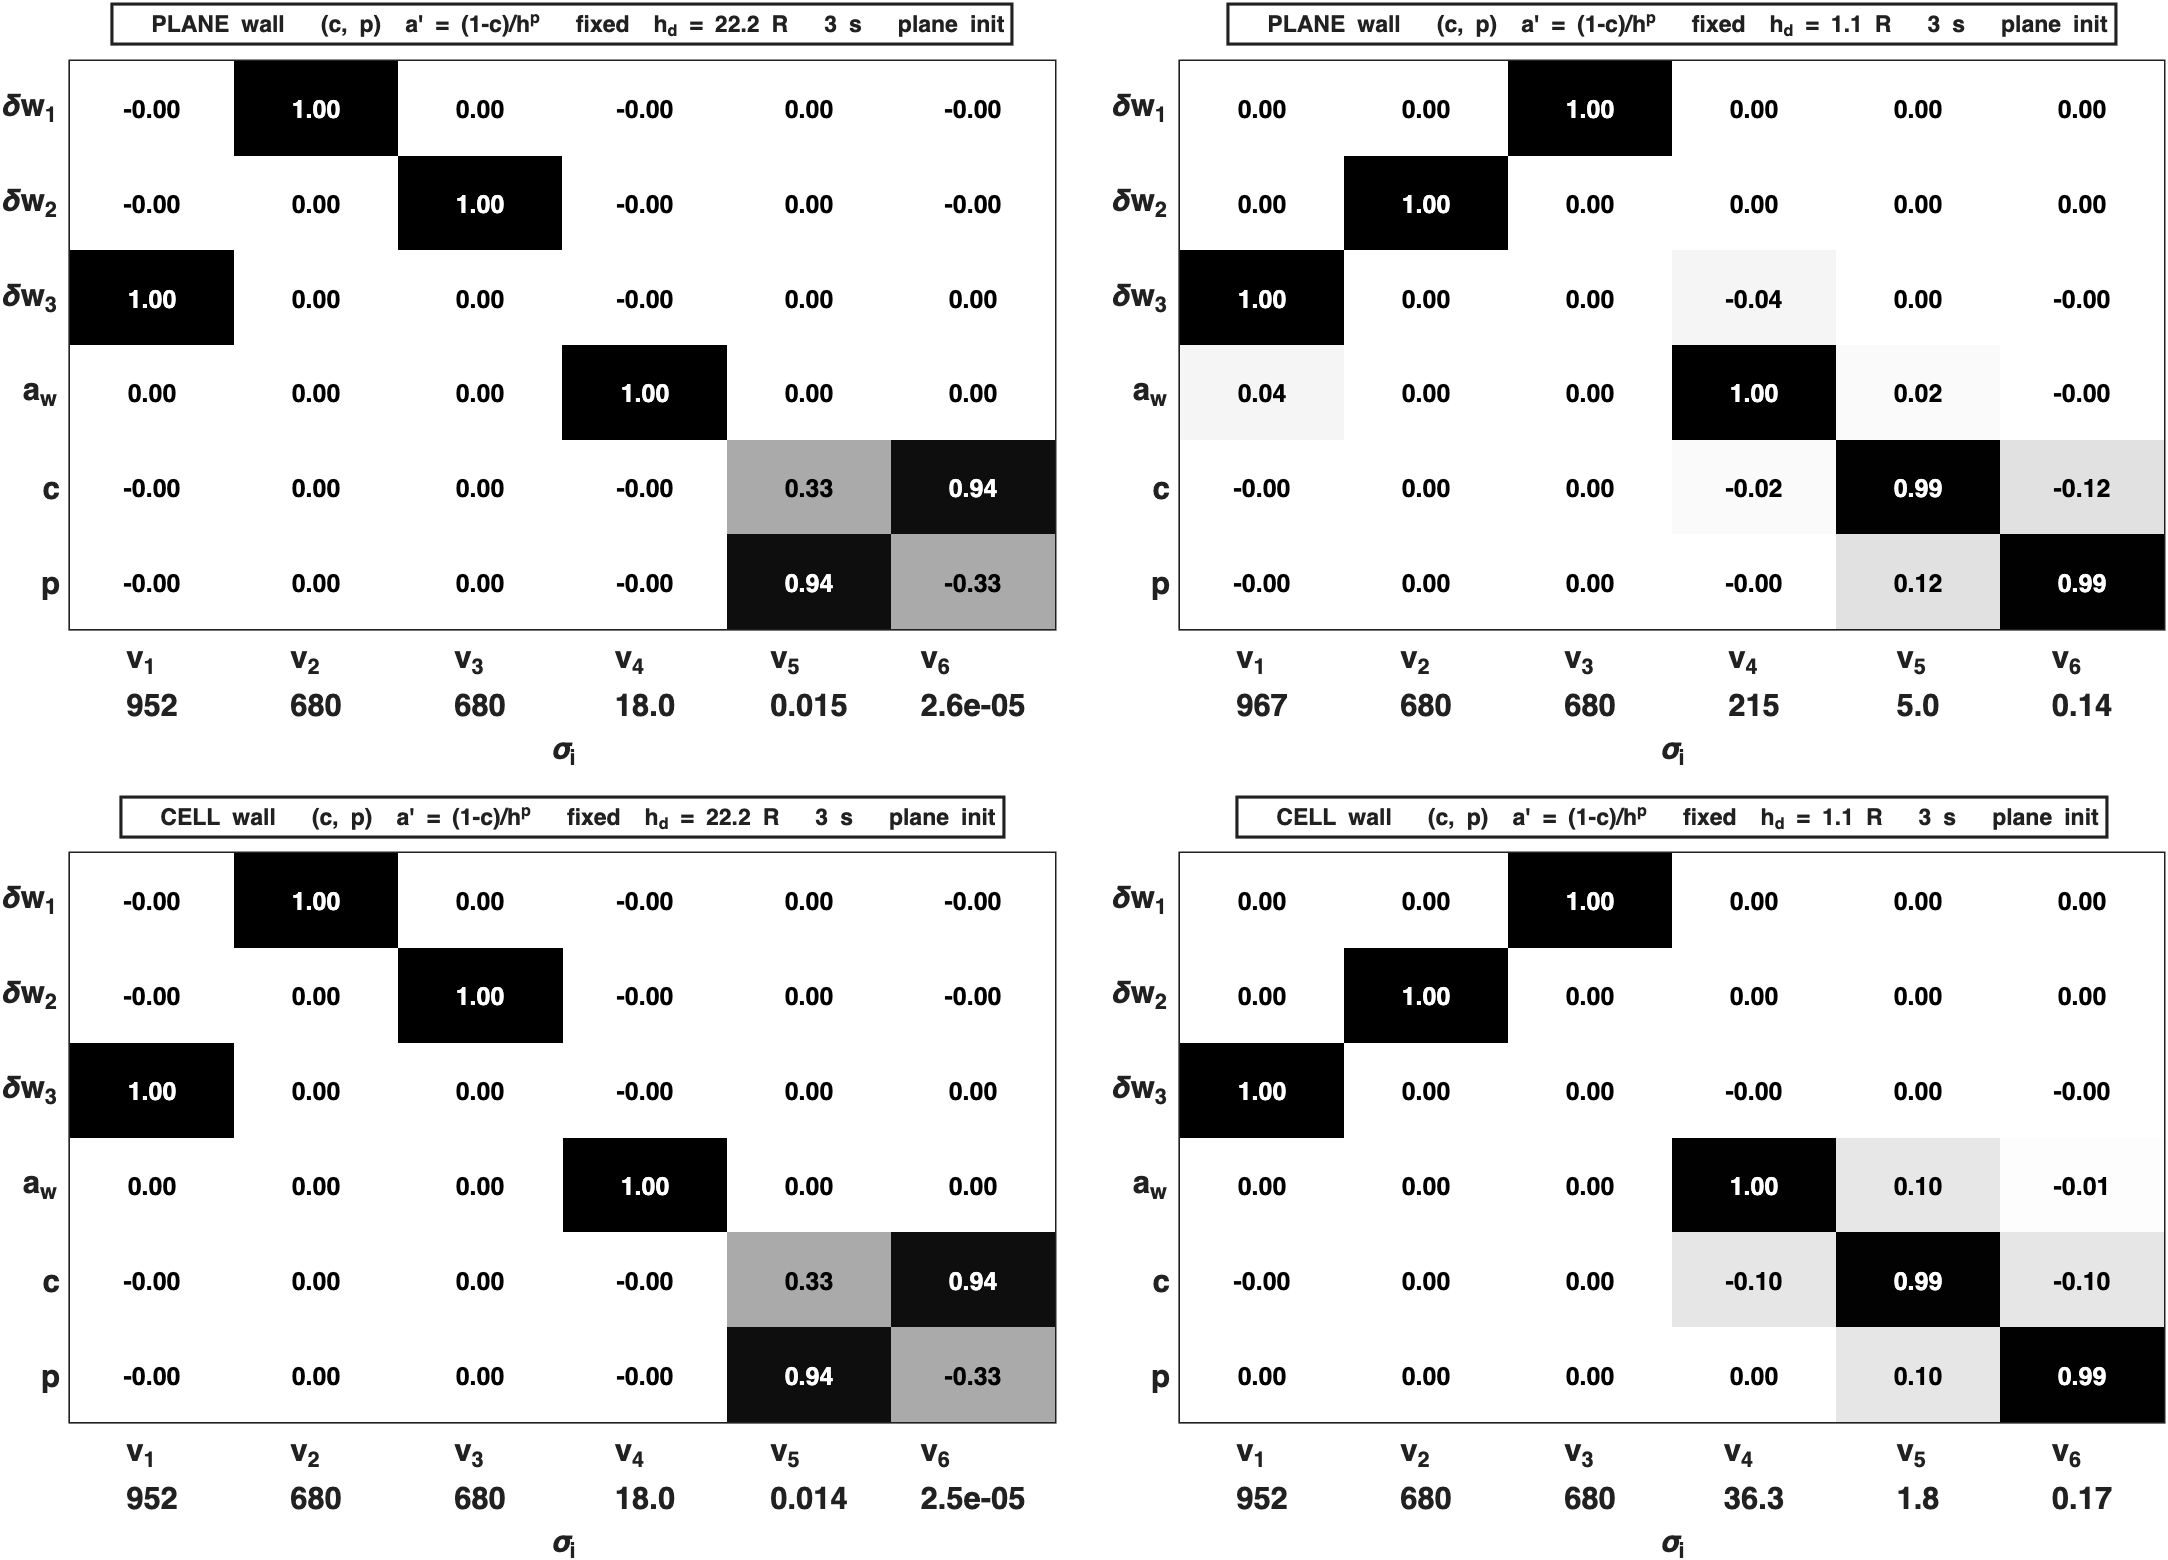
\includegraphics[width=\textwidth]{obs_fixed_V_f1.png}\end{center}

\clearpage
\section{Slope law $a'(h;\,c,p)$, both constants estimated, $T_d = 2$ s: observability over the descent}

Plane and cell wall, plane init, one seed.
\begin{align*}
a[k+1] &= a[k] + a'(h_d[k];\,c,p)\,\Delta h_d[k], \qquad a' = \frac{1-c}{h^p} \\
c[k+1] &= c[k] \\
p[k+1] &= p[k]
\end{align*}

\begin{center}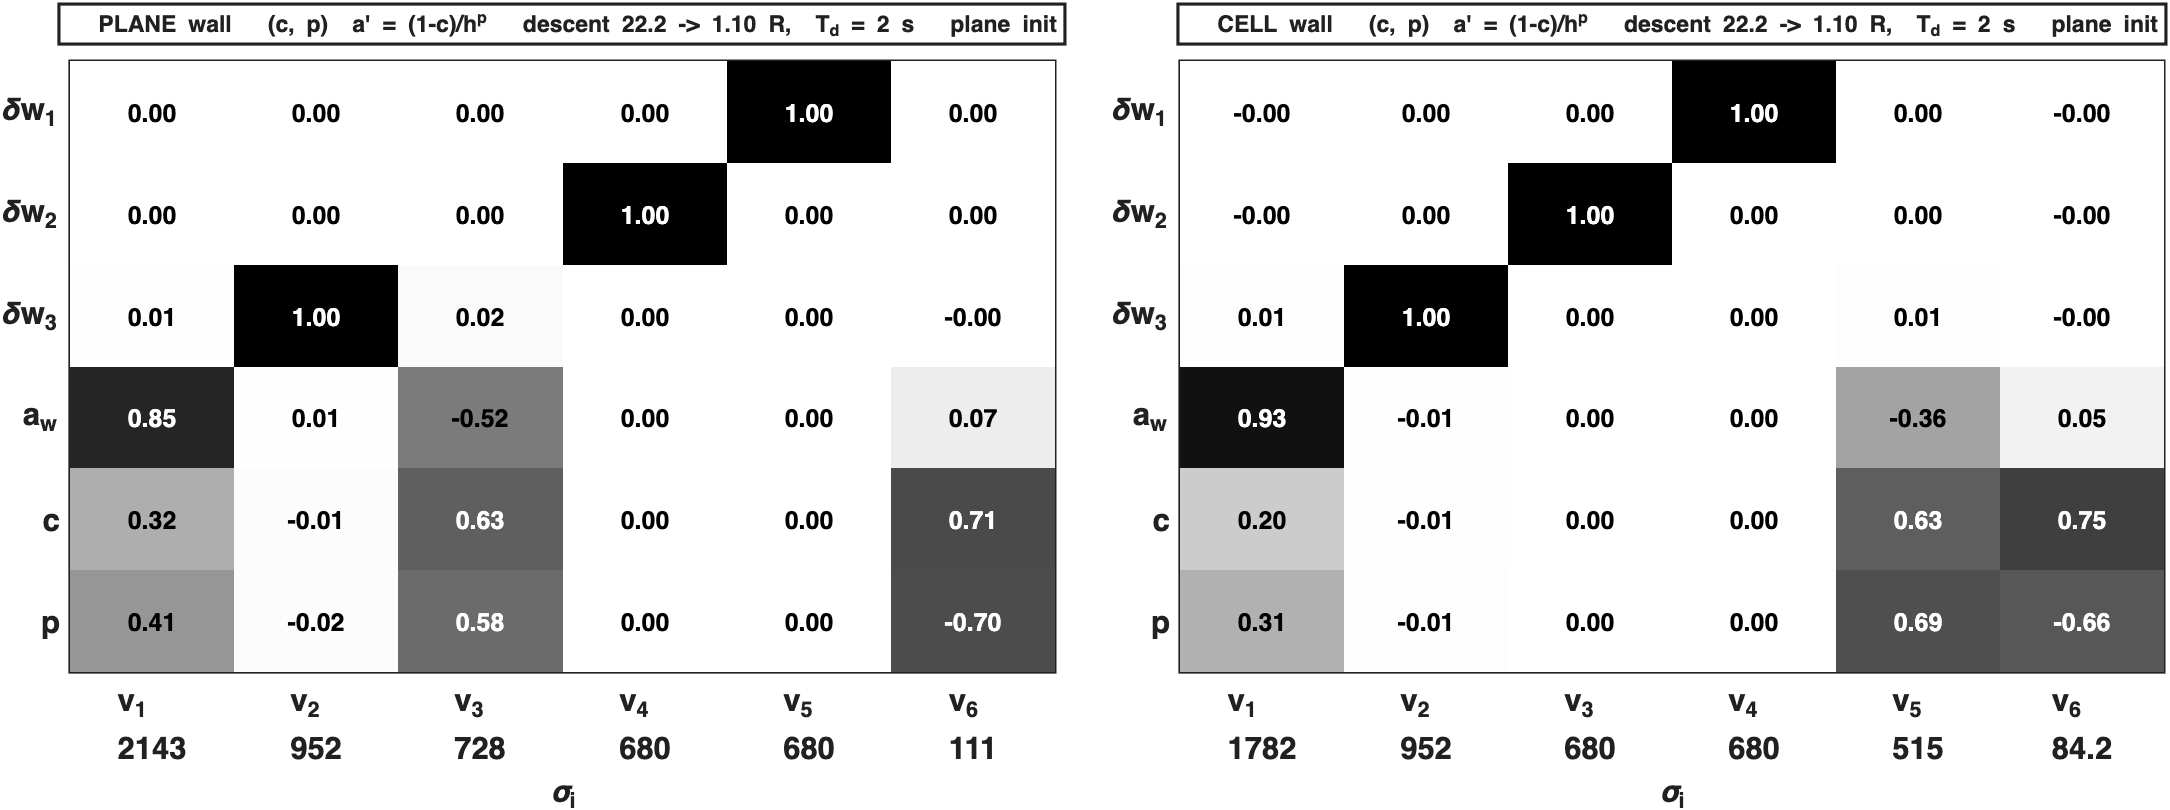
\includegraphics[width=\textwidth]{obs_ramp_f1_V_Td2.png}\end{center}

\clearpage
\section{Slope law $a'(h;\,c,p)$, both constants estimated, $T_d = 2$ s: plane and cell wall}

Plane init, 10 seeds.
\begin{align*}
a[k+1] &= a[k] + a'(h_d[k];\,c,p)\,\Delta h_d[k], \qquad a' = \frac{1-c}{h^p} \\
c[k+1] &= c[k] \\
p[k+1] &= p[k]
\end{align*}

\begin{center}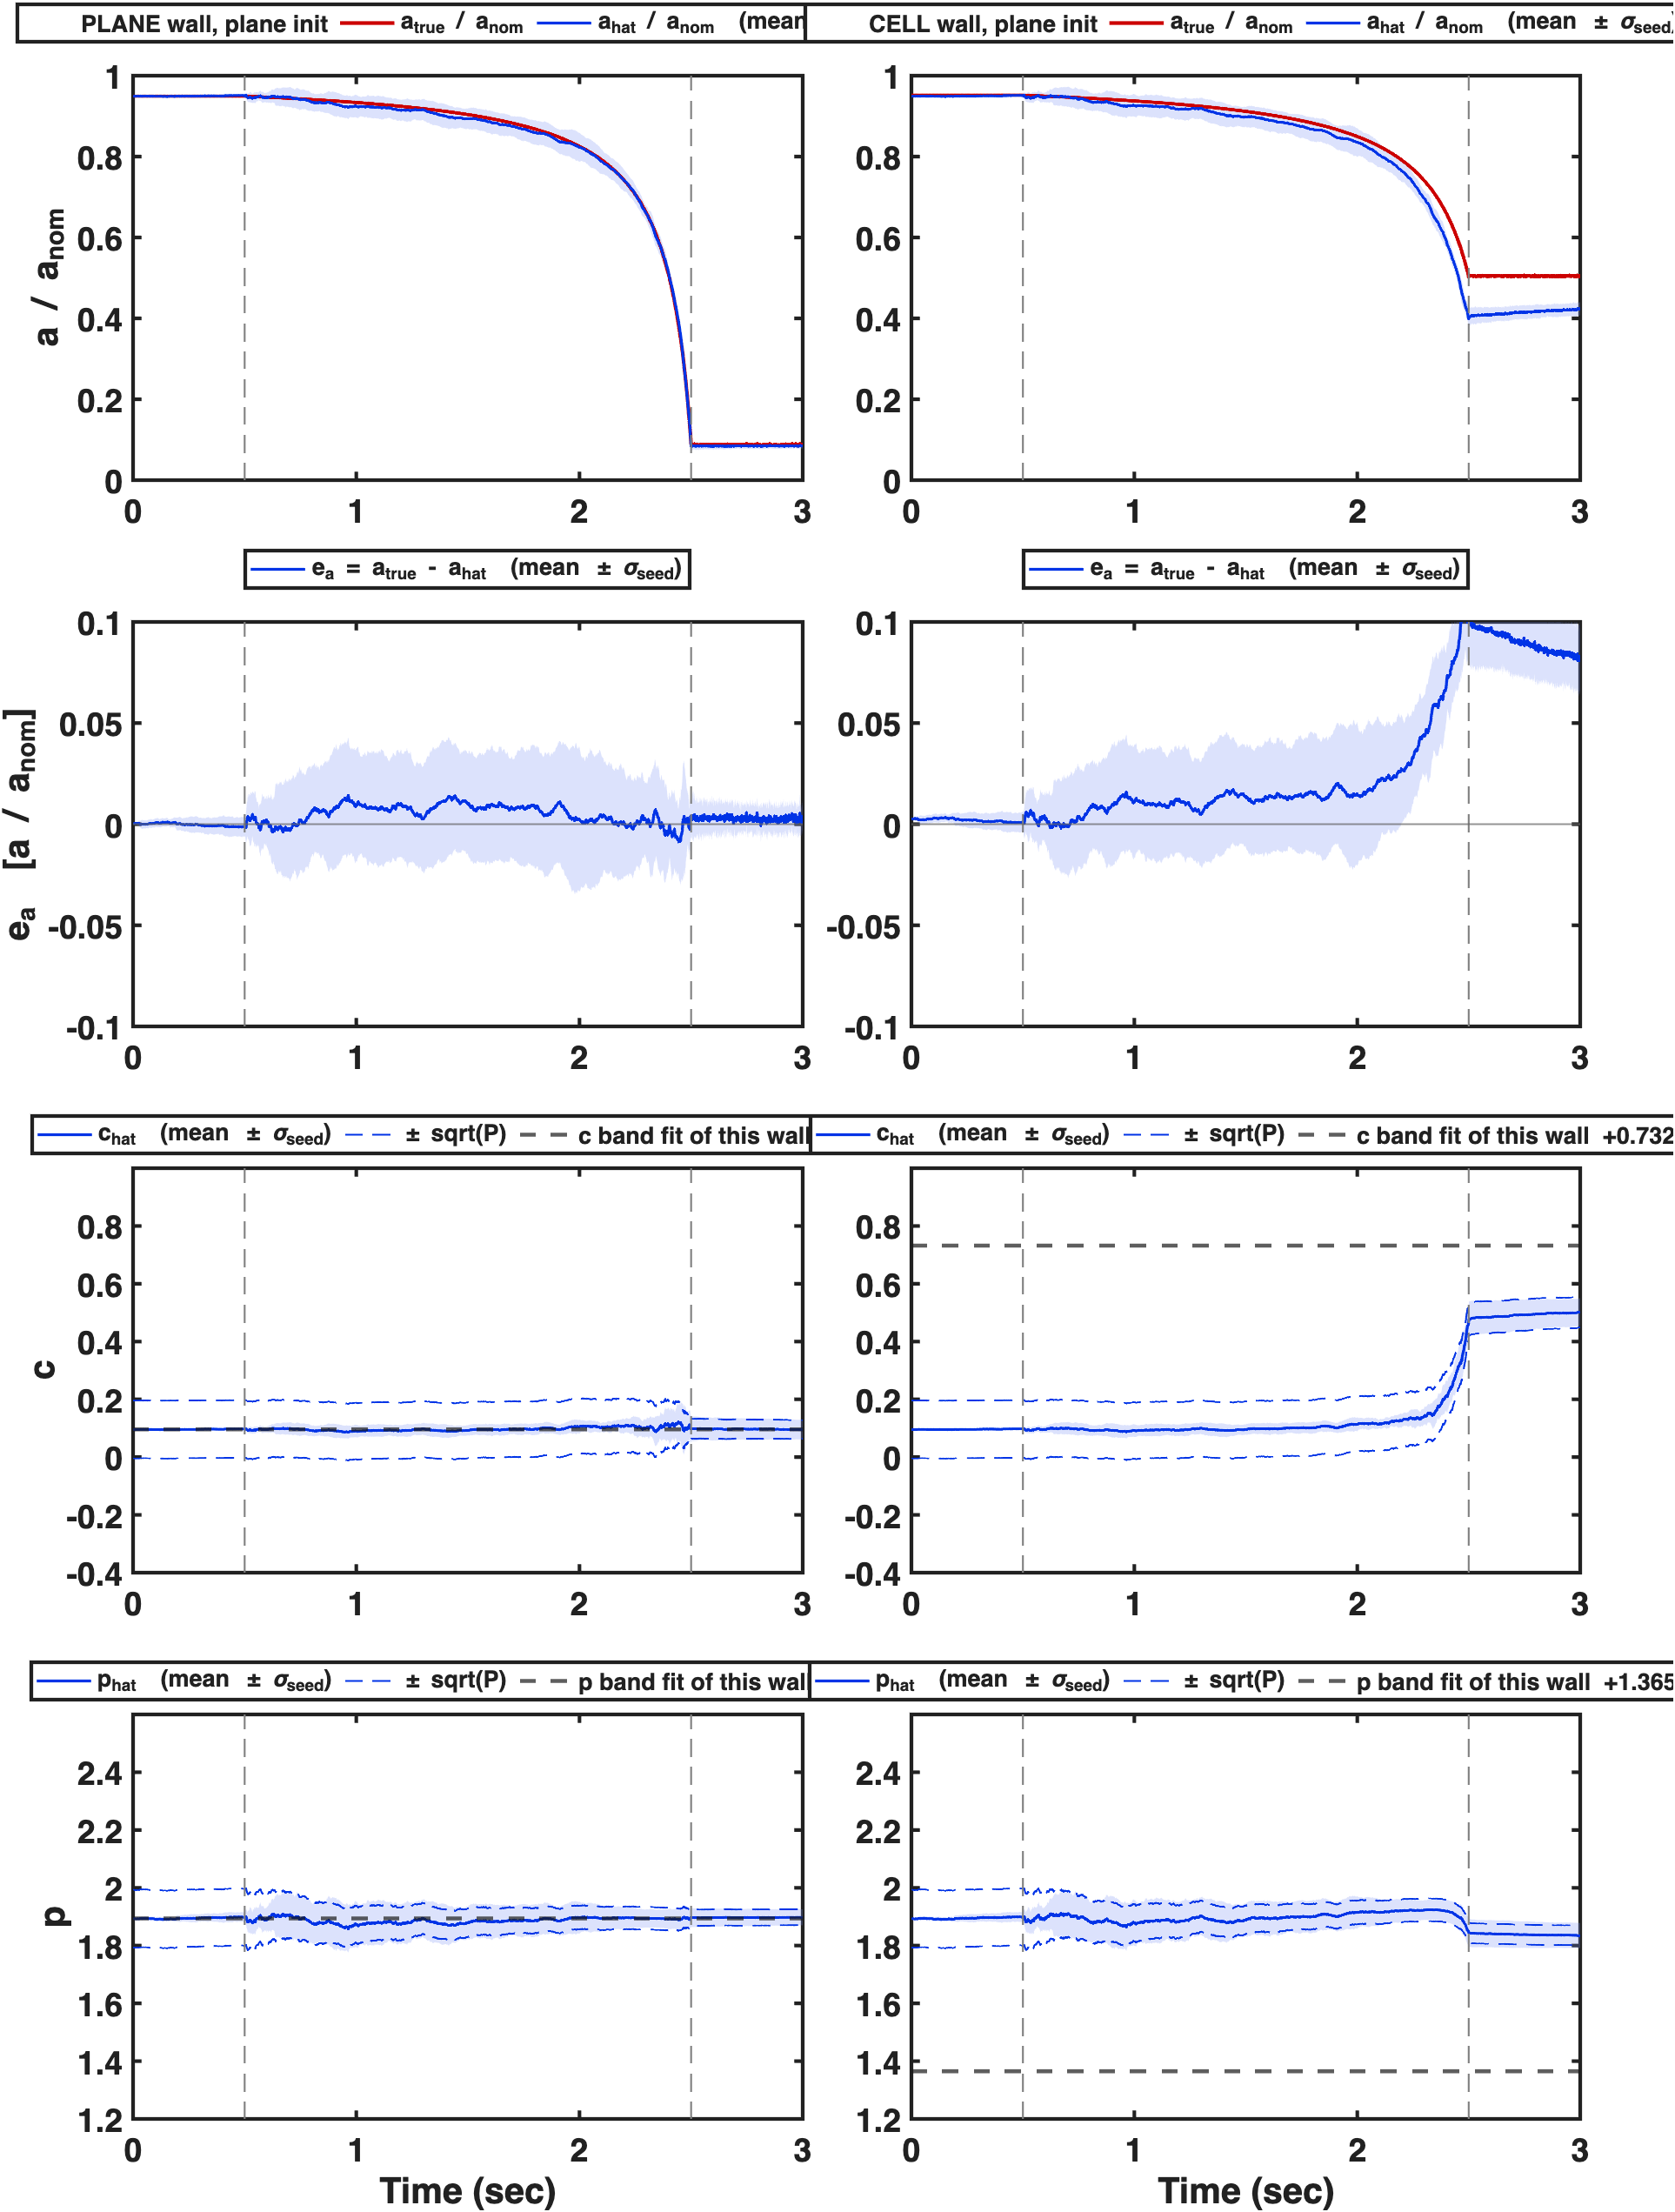
\includegraphics[width=\textwidth,height=0.78\textheight,keepaspectratio]{f1_walls_PI_ramp2.png}\end{center}

\clearpage
\section{Slope law $a'(h, c)$, $p = 2$, one constant, $T_d = 2$ s: observability over the descent}

Plane and cell wall, plane init $c = 0.053$, one seed. $\sigma_i$, $v_i$ as in Section 3; $p$ known, so it is not a state.
\begin{align*}
a[k+1] &= a[k] + a'(h_d[k], c)\,\Delta h_d[k], \qquad a' = \frac{1-c}{h^2} \\
c[k+1] &= c[k]
\end{align*}

\begin{center}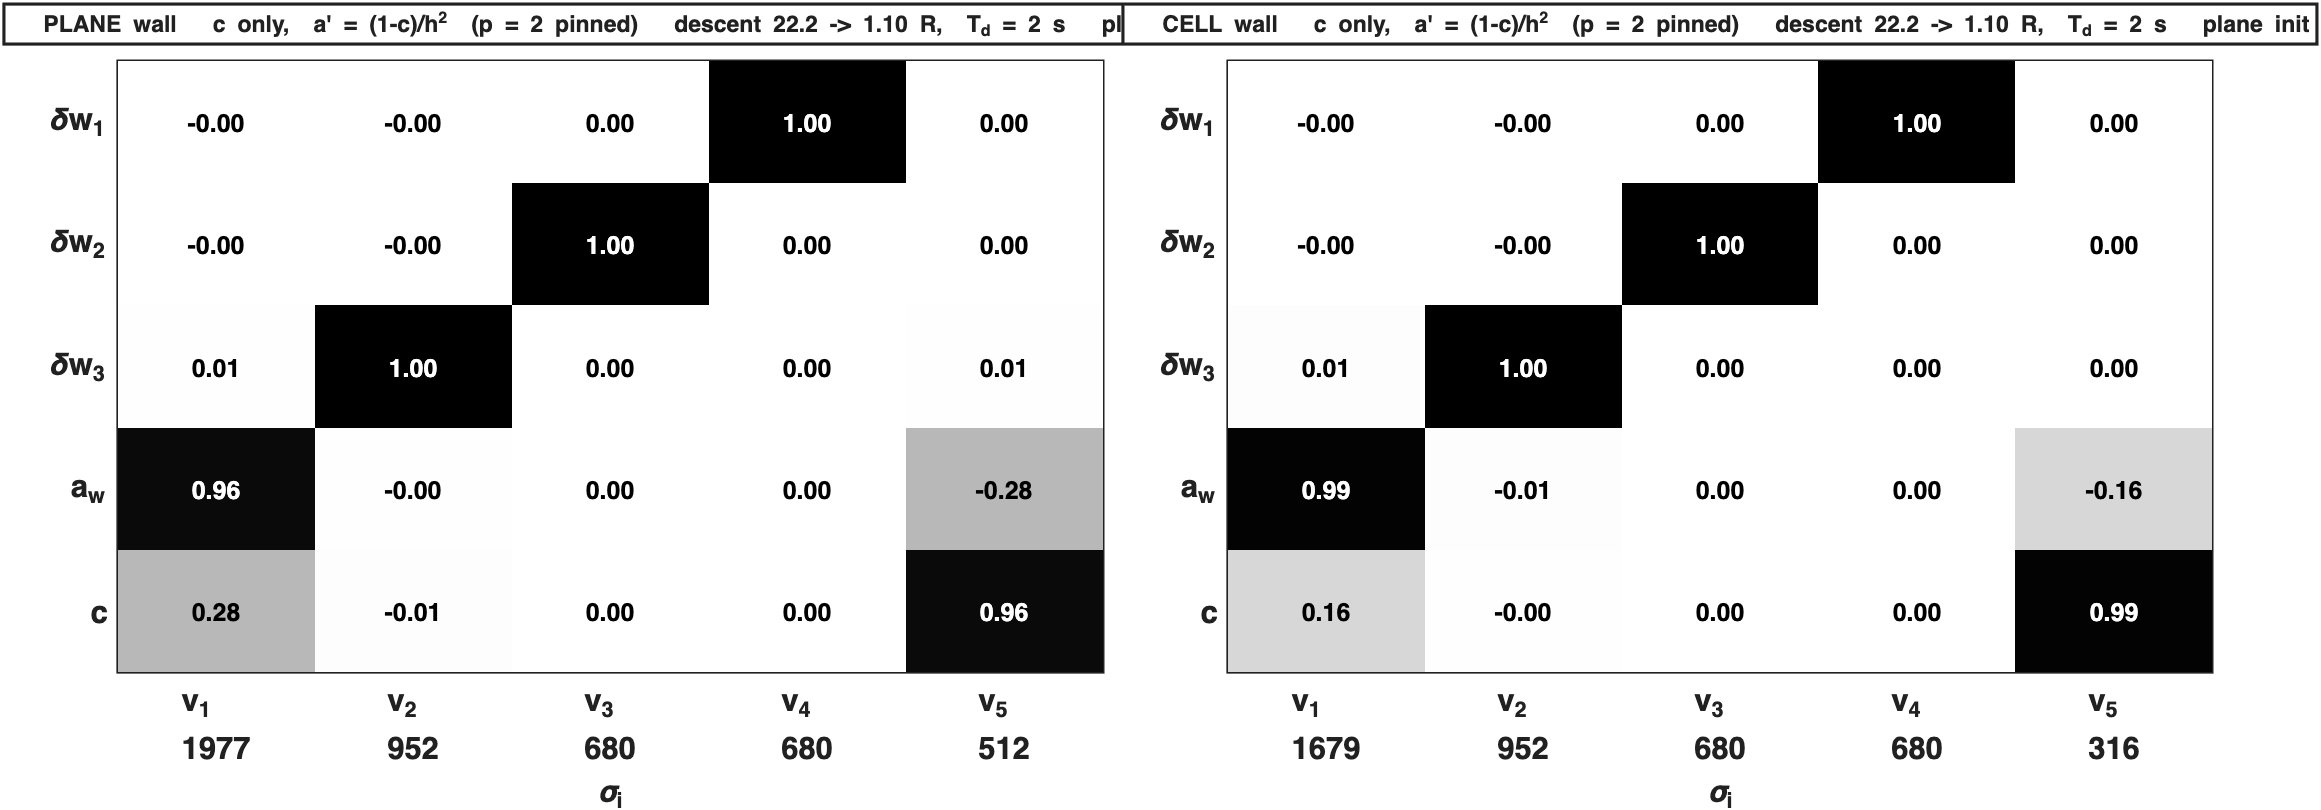
\includegraphics[width=\textwidth]{obs_ramp_f1p2_V_Td2.png}\end{center}

\clearpage
\section{Slope law $a'(h, c)$, $p = 2$, one constant, $T_d = 2$ s: plane and cell wall}

Plane init $c = 0.053$ (plane band fit at $p = 2$), prior 0.10, 10 seeds, $\lambda_f = 1$.
\begin{align*}
a[k+1] &= a[k] + a'(h_d[k], c)\,\Delta h_d[k], \qquad a' = \frac{1-c}{h^2} \\
c[k+1] &= c[k]
\end{align*}

\begin{center}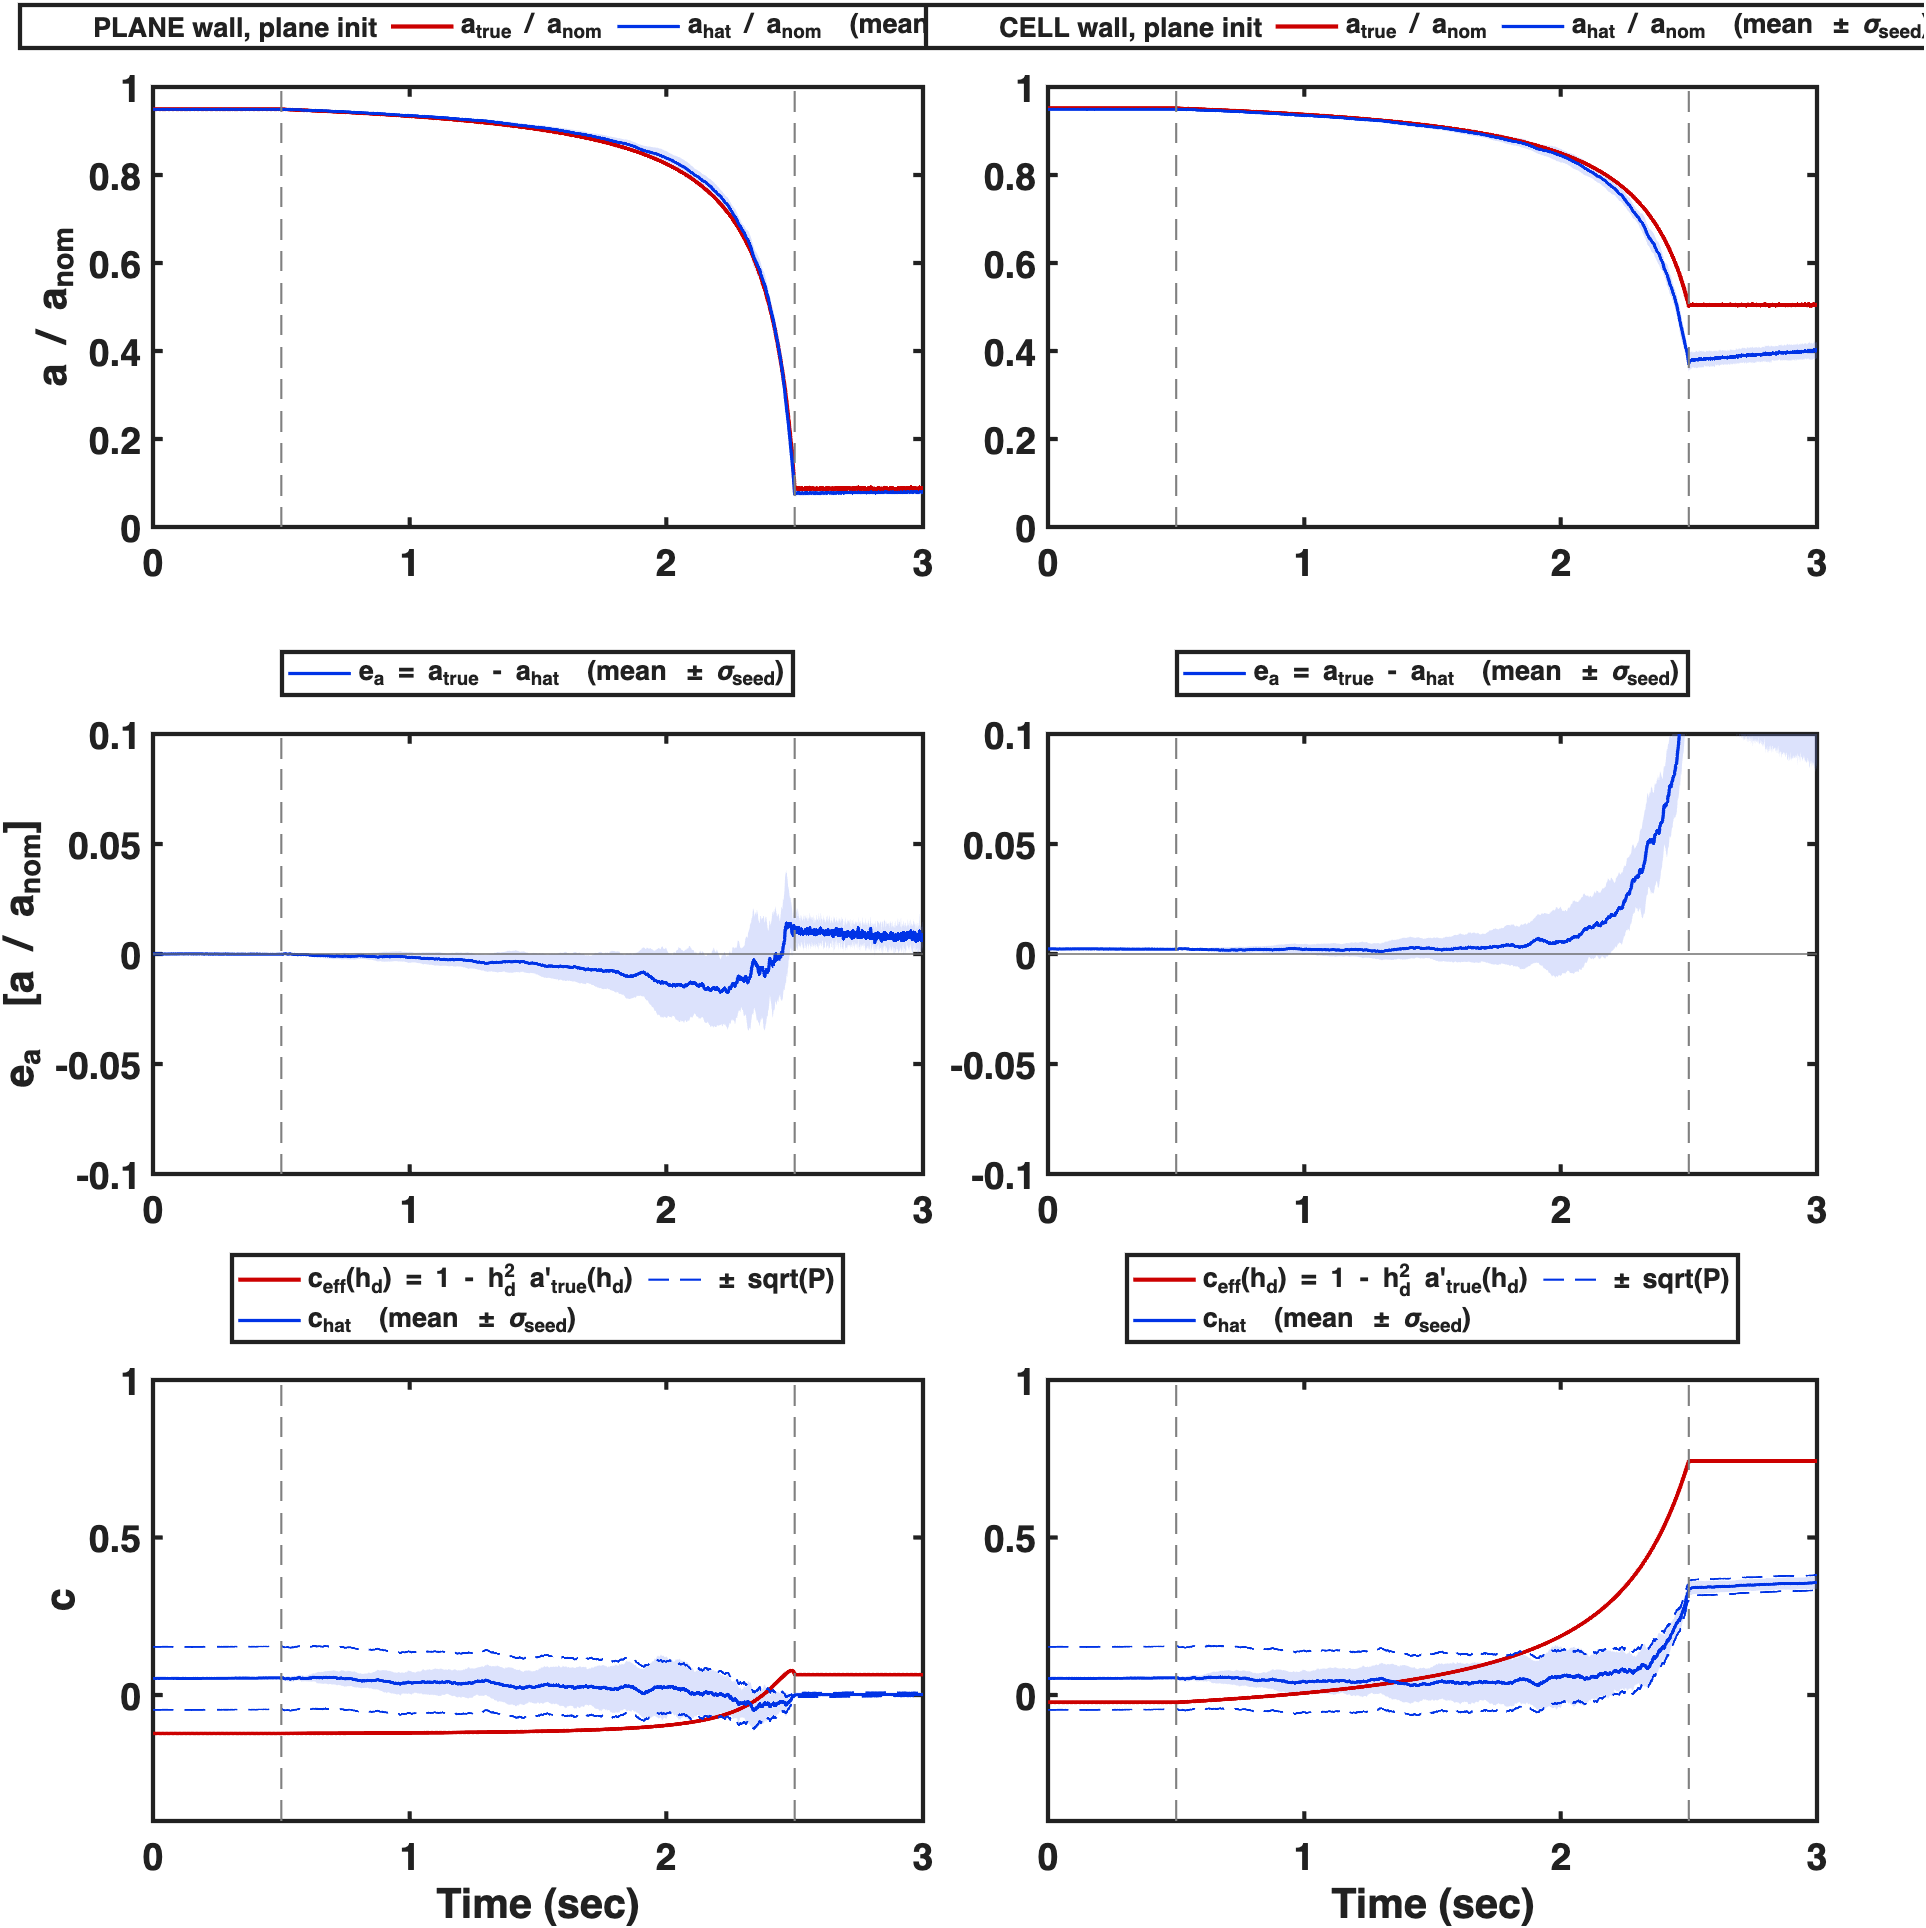
\includegraphics[width=\textwidth,height=0.78\textheight,keepaspectratio]{f1p2_walls_PI_sig010_ramp2.png}\end{center}

\clearpage
\section{Covariance recursion: the update only shrinks $P$; where the forgetting factor enters}

Kalman filter, one step (Meng 2025 (19)--(21)); $c$ a constant state, $Q_{cc} = 0$. No measurement value appears in (19)--(21).
\begin{align*}
L &= P^f H^T \left(H P^f H^T + R\right)^{-1} \\
P &= (I - LH)\,P^f \;=\; P^f - P^f H^T \left(H P^f H^T + R\right)^{-1} H P^f \;\le\; P^f \\
P^f[k+1] &= F_e\, P\, F_e^T + Q, \qquad Q_{cc} = 0 \;\Rightarrow\; P^f_{cc}[k+1] = P_{cc}[k]
\end{align*}
The same step for the $c$ element, written in information ($1/P_{cc}$):
\begin{align*}
s_k &= 1 - \frac{P_{cc}[k]}{P^f_{cc}[k]} \qquad\text{(fraction of } c\text{'s variance removed by this update; set by } P^f, H, R \text{ only)} \\
\frac{1}{P_{cc}[k]} &= \frac{1}{P_{cc}[k-1]} + g_k, \qquad g_k = \frac{s_k}{(1 - s_k)\,P^f_{cc}[k]}
\end{align*}
Forgetting on the $c$ element only (after the update, before the next prediction):
\begin{align*}
P_{cc} &\leftarrow P_{cc}/\lambda_k, \quad P_{cj} \leftarrow P_{cj}/\sqrt{\lambda_k}
\qquad\Leftrightarrow\qquad
\frac{1}{P_{cc}[k]} = \lambda_k \left(\frac{1}{P_{cc}[k-1]} + g_k\right) \\
\lambda_k &= 1 \;\text{(constant)}, \qquad \lambda_k = \lambda_f \;\text{(uniform)}, \qquad \lambda_k = \exp(-\beta\, s_k) \;\text{(information-driven)} \\
\lambda_k &= \exp(-\beta\, s_k) \;\Rightarrow\; (1 - \lambda_k)\left(\frac{1}{P_{cc}[k-1]} + g_k\right) \approx \beta\, g_k
\end{align*}

\clearpage
\section{Slope law $a'(h, c)$, $p = 2$, one constant, $T_d = 2$ s: cell wall, three forgetting factors on $c$}

Plane init $c = 0.053$, prior 0.10, 10 seeds. Forgetting on the $c$ element after each update (Section 8), one choice per column.
\begin{align*}
a[k+1] &= a[k] + a'(h_d[k], c)\,\Delta h_d[k], \qquad a' = \frac{1-c}{h^2} \\
c[k+1] &= c[k] \\
P_{cc} &\leftarrow P_{cc}/\lambda_k, \qquad P_{cj} \leftarrow P_{cj}/\sqrt{\lambda_k} \\
\text{left:}\quad \lambda_k &= \max\{\exp(-3\, s_k),\; 0.99\}, \qquad s_k = 1 - \frac{P_{cc}[k]}{P^f_{cc}[k]} \\
\text{middle:}\quad \lambda_k &= 0.999 \\
\text{right:}\quad \lambda_k &= 1
\end{align*}

\begin{center}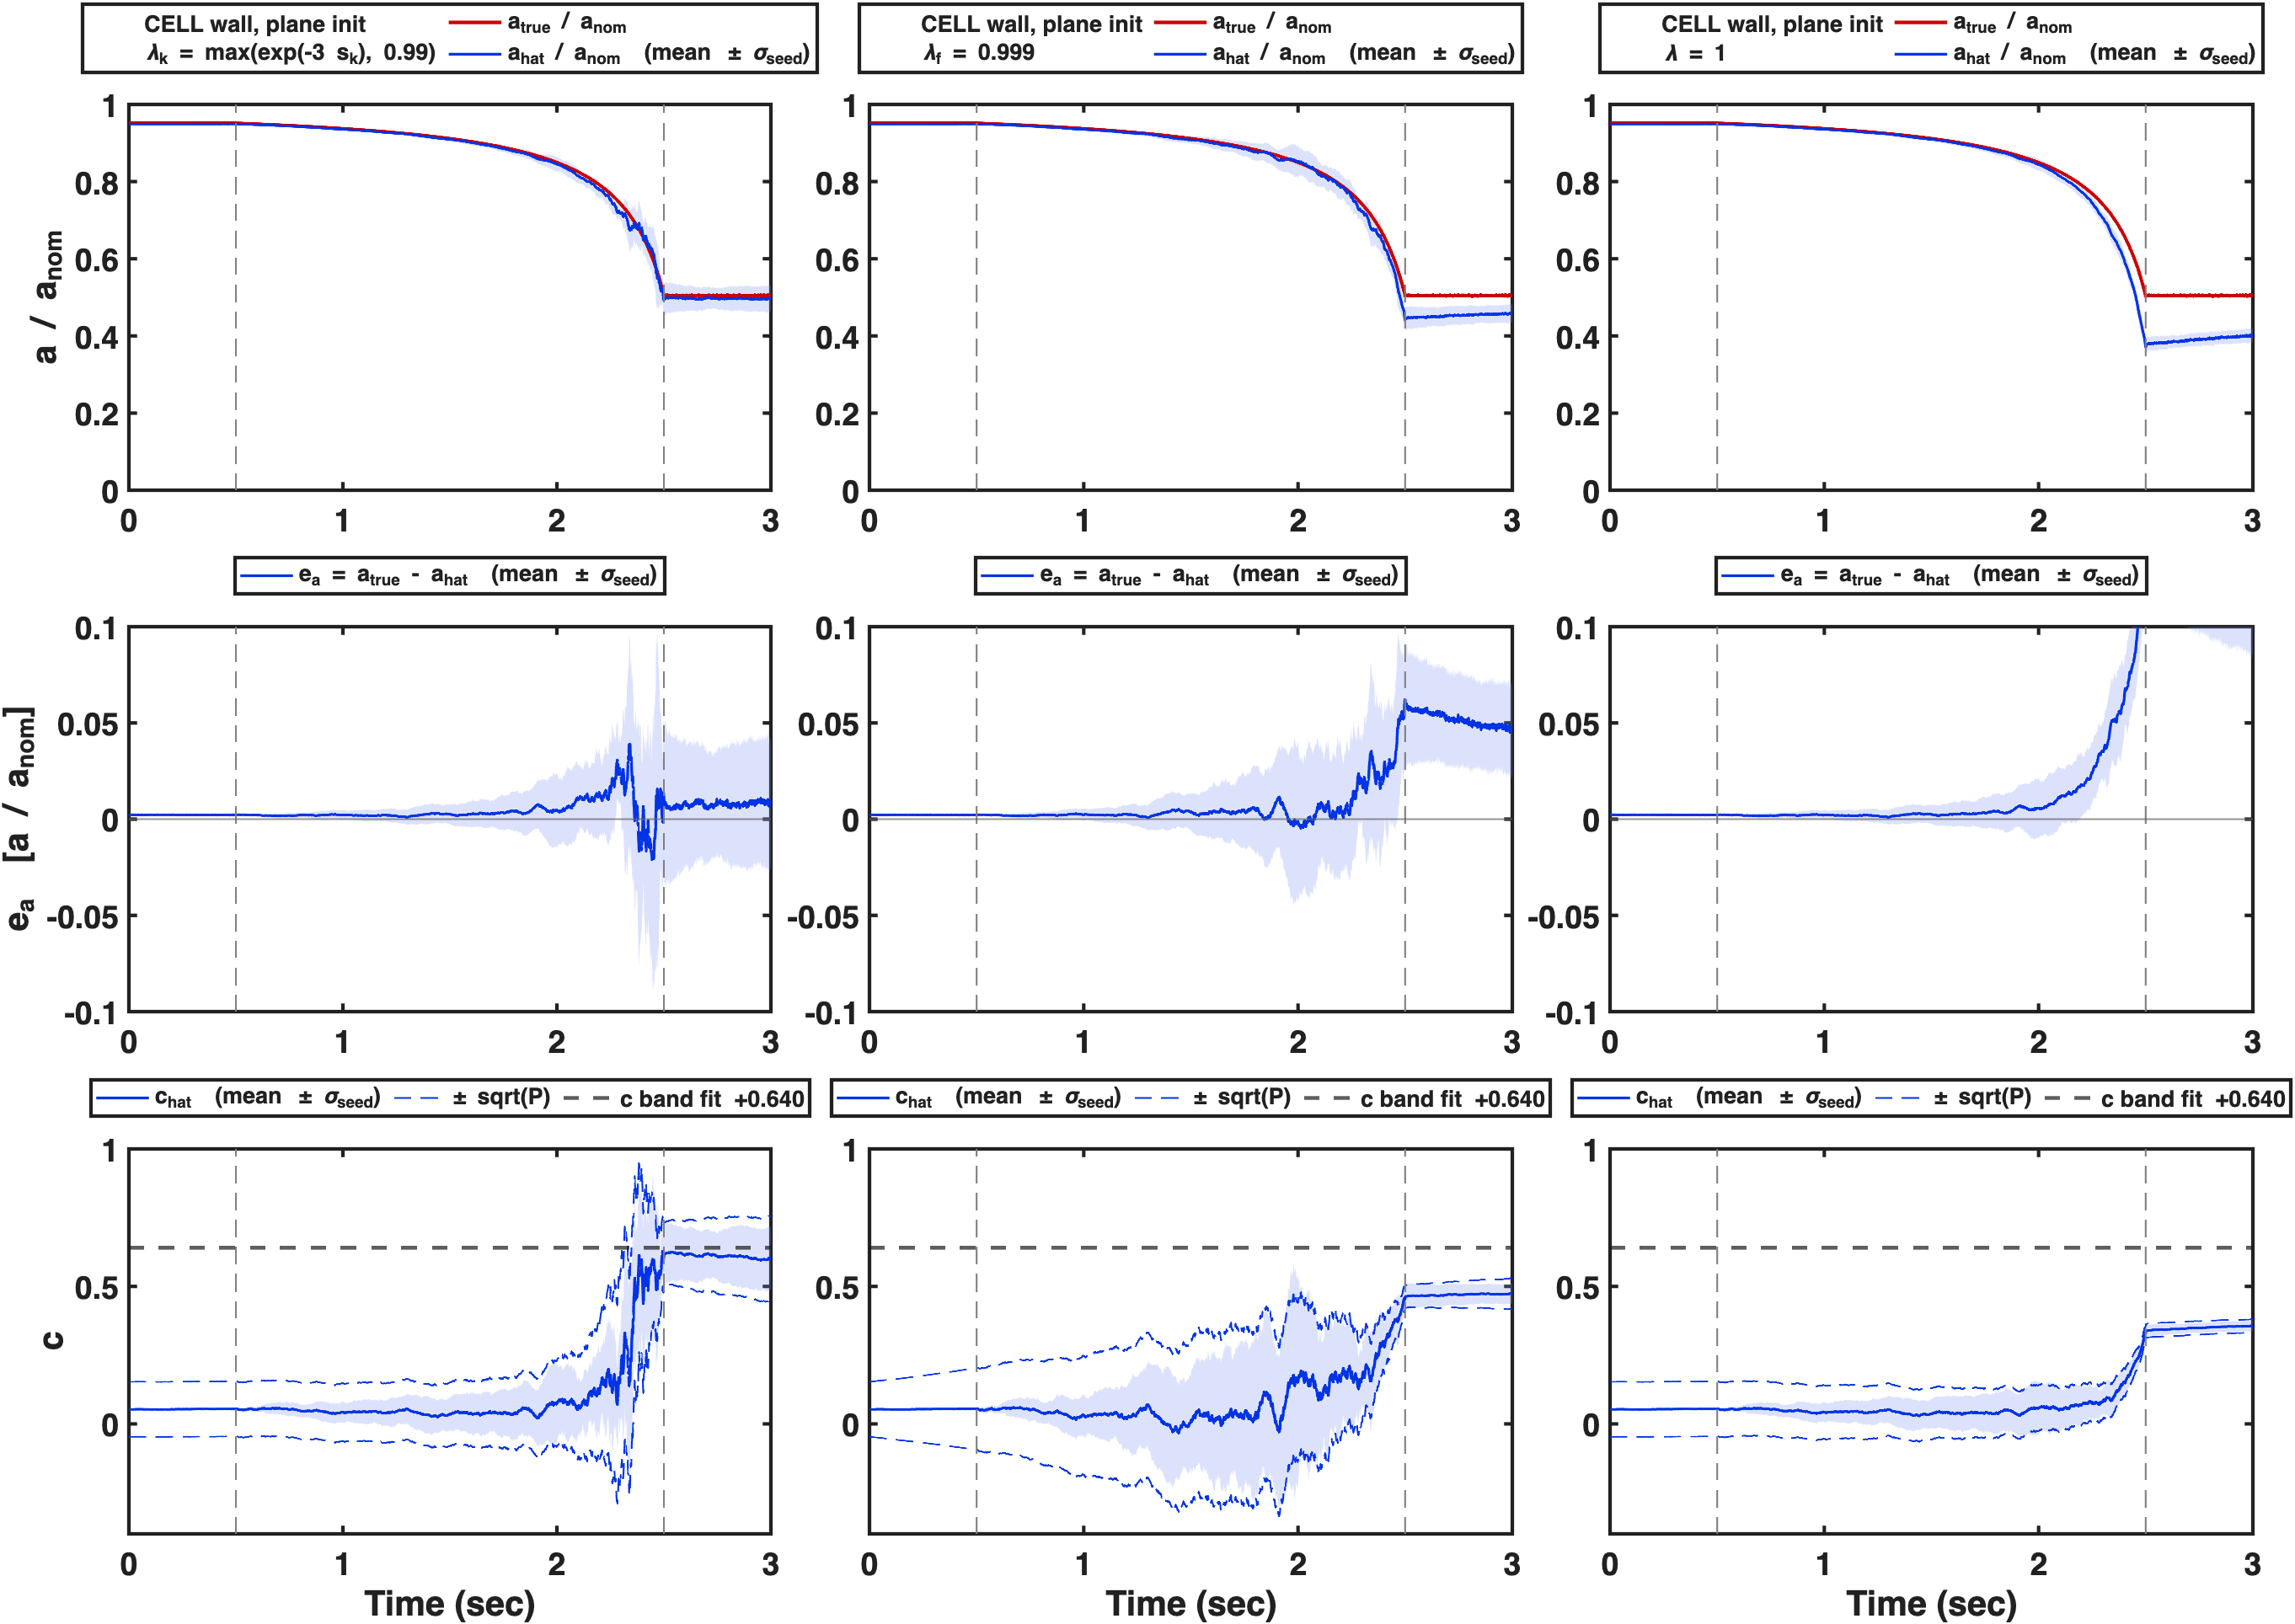
\includegraphics[width=\textwidth,height=0.78\textheight,keepaspectratio]{f1p2_cell_lf_compare.png}\end{center}

\end{document}
